\documentclass[a4paper,11pt]{article}
\usepackage{amssymb, enumitem}


\parindent 0cm
\usepackage{amssymb,amsmath,amsthm,latexsym,epsfig,euscript,multicol}
\usepackage{graphbox}

\usepackage[utf8x]{inputenc}
\usepackage{listings,xcolor,bm}


\definecolor{mygreen}{rgb}{0,0.6,0}
\definecolor{mygray}{rgb}{0.5,0.5,0.5}
\definecolor{mymauve}{rgb}{0.58,0,0.82}
\lstset{
  backgroundcolor=\color{white},   % choose the background color; you must add
  basicstyle=\small\ttfamily,      % the size of the fonts that are used for the code
  breakatwhitespace=false,         % sets if automatic breaks should only happen at whitespace
  breaklines=true,                 % sets automatic line breaking
  captionpos=b,                    % sets the caption-position to bottom
  commentstyle=\color{mygreen},    % comment style
  deletekeywords={...},            % if you want to delete keywords from the given language
  escapeinside={\%*}{*)},          % if you want to add LaTeX within your code
  extendedchars=true,              % lets you use non-ASCII characters; for 8-bits encodings only, does not work with UTF-8
  firstnumber=1,                % start line enumeration with line 1000
  frame=single,	                   % adds a frame around the code
  keepspaces=true,                 % keeps spaces in text, useful for keeping indentation of code (possibly needs columns=flexible)
  keywordstyle=\color{blue},       % keyword style
  language=Python,                 % the language of the code
  morekeywords={*,...},            % if you want to add more keywords to the set
  numbers=left,                    % where to put the line-numbers; possible values are (none, left, right)
  numbersep=5pt,                   % how far the line-numbers are from the code
  numberstyle=\tiny\color{mygray}, % the style that is used for the line-numbers
  rulecolor=\color{black},         % if not set, the frame-color may be changed on line-breaks within not-black text (e.g. comments (green here))
  showspaces=false,                % show spaces everywhere adding particular underscores; it overrides 'showstringspaces'
  showstringspaces=false,          % underline spaces within strings only
  showtabs=false,                  % show tabs within strings adding particular underscores
  stepnumber=5,                    % the step between two line-numbers. If it's 1, each line will be numbered
  stringstyle=\color{mymauve},     % string literal style
  tabsize=4,	                   % sets default tabsize to 2 spaces
  title=\lstname                   % show the filename of files included with \lstinputlisting; also try caption instead of title
}
% Caracteres especiales
\def\A{\mathbb{A}}
\def\C{\mathbb{C}}
\def \N{\mathbb{N}}
\def \P{\mathbb{P}}
\def \Q{\mathbb{Q}}
\def \R{\mathbb{R}}
\def \Z{\mathbb{Z}}
\def \sen{\textrm{sen}}

\def\Np{$\N$}
\def\Zp{$\Z$}
\def\Qp{$\Q$}
\def\Rp{$\R$}
\def\Cp{$\C$}

\def\bb{\bm{b}}
\def\bu{\bm{u}}
\def\bv{\bm{v}}
\def\bx{\bm{x}}
\def\bA{\bm{A}}
\def\bB{\bm{B}}
\def\bD{\bm{D}}
\def\bE{\bm{E}}
\def\bM{\bm{M}}
\def\bT{\bm{T}}


\def\K{\textrm{K}}
\def\V{\textrm{V}}
\def\S{\textrm{S}}

\def\degres{$^\circ$}

\newcount\todno
\def\no{\global\advance\todno by 1 \the\todno}

\topmargin-2cm \vsize 29.5cm \hsize 21cm
\setlength{\textwidth}{16.75cm}\setlength{\textheight}{23.5cm}
\setlength{\oddsidemargin}{0.0cm}
\setlength{\evensidemargin}{0.0cm}


\theoremstyle{definition}
\newtheorem{ejer}{Ejercicio}
\newcommand{\bej}{\begin{ejer}}
\newcommand{\fej}{\end{ejer}}

\begin{document}

\centerline{{\small Universidad de Buenos Aires - Facultad de Ciencias Exactas y Naturales - Ciencias de Datos}}

\vskip 0.2cm

\hrule

\vskip 0.2cm

 \centerline{{\bf\Large{\sc Laboratorio de Datos}}}

 \vskip 0.2cm

 \centerline{\ttfamily Primer Cuatrimestre 2024}

\vskip 0.2cm

 \hrule

 \bigskip
 \centerline{\bf Práctica N$^\circ$ 3: Visualizaci\'on de datos.}
 \bigskip


% \textbf{\large Visualizaci\'on}

\begin{enumerate}[resume]
\item Ten\'es datos de una encuesta realizada en distintas provincias de Argentina y quer\'es saber cu\'antas personas respondieron a la encuesta en cada provincia. ?`Hac\'es un gr\'afico de l\'ineas, de dispersi\'on (scatter), histograma o un gr\'afico de barras (bar plot)? Hac\'e a mano en tu cuaderno c\'omo esper\'as que se vea el gr\'afico.

\item Est\'as estudiando la relaci\'on entre altura y peso de las personas. Ten\'es un data-set que tiene como variables la edad, sexo y peso de cada persona. Si quer\'es describir estas variables por separado, ?`qu\'e gr\'afico har\'ias para cada una? ?`y si quer\'es visualizar la relaci\'on entre peso y altura? Hac\'e a mano en tu cuaderno c\'omo esper\'as que se vea el gr\'afico.

\item Hac\'e un gr\'afico de barras que muestre la cantidad de pa\'ises hay en cada continente seg\'un los datos de gapminder (recordar el ejercicio 10 de la Práctica 2 para acceder a los datos de gapminder).

\item Quer\'es investigar c\'omo var\'ia la expectativa de vida entre los continentes. Para eso necesit\'as un gr\'afico como el siguiente:

\begin{center}
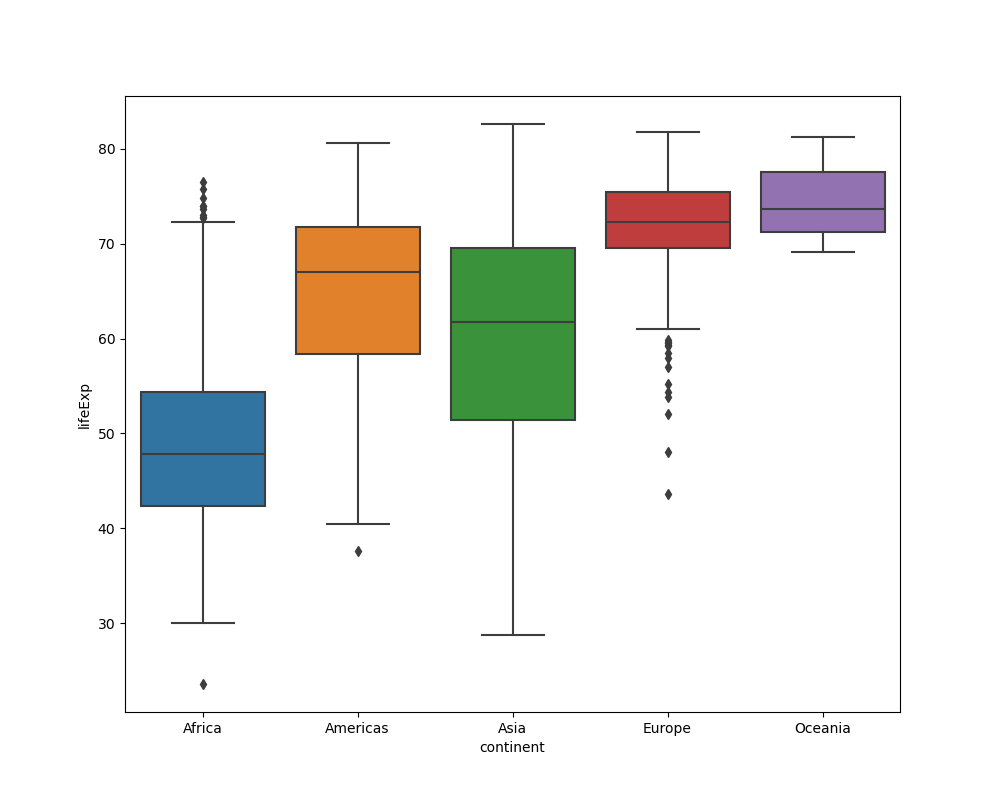
\includegraphics[scale=0.6]{practica3-img-gapminder-boxplot.png}
\end{center}

Reproduc\'i el gr\'afico de arriba reemplazando adecuadamente lo que falta en el siguiente c\'odigo:
\begin{lstlisting}
import seaborn as sns
sns.boxplot(gapminder, x=COMPLETAR, y=COMPLETAR, order=sorted(COMPLETAR))
\end{lstlisting}

\item
\begin{enumerate}
\item Utilizando \lstinline{seaborn.objects}, graficar la curva de la expectativa de vida en Argentina en función del año, completando el siguiente código. Sugerencia: recordar de la práctica anterior como filtrar datos de un dataset.

\begin{lstlisting}
import seaborn.objects as so
(
    so.Plot(data = gapminder[???], x = "year", y = "???")
    .add(so.Line())
)
\end{lstlisting}
    
    
\item Realizar un nuevo gráfico donde puedan verse las curvas de la expectativa de vida de los países de América en función del año, una curva por cada país.

    Sugerencia: utilizar los parámetros \lstinline{group = ???} o \lstinline{color = ???}. ¿Cuál es la diferencia entre los dos?
\item \label{ej:map} Queremos agregar al gráfico del ítem anterior una curva de tendencia lineal utilizando el método  \lstinline{.add(so.Line(), so.PolyFit(1))}. ¿Cuál de las siguientes dos formas de agrupar los datos es la forma correcta? Explicar la diferencia entre los dos códigos.

\begin{lstlisting}
# Codigo 1
(
    so.Plot(data = ???, x=???, y=???, group = ???)
    .add(so.Lines(color="#bbca"))
    .add(so.Line(), so.PolyFit(1))
)

# Codigo 2
(
    so.Plot(data = ???, x=???, y=???)
    .add(so.Lines(color="#bbca"), group = ???)
    .add(so.Line(), so.PolyFit(1))
)
\end{lstlisting}

\item Realizar el siguiente gráfico, con las curvas de expectativa de vida agrupadas por continente. Sugerencias: ¿qué hace el método \lstinline{facet()} de \lstinline{seaborn.objects.Plot()}? ?`Y el parámetro \lstinline{wrap = ???} de \lstinline{facet()}?
\begin{center}
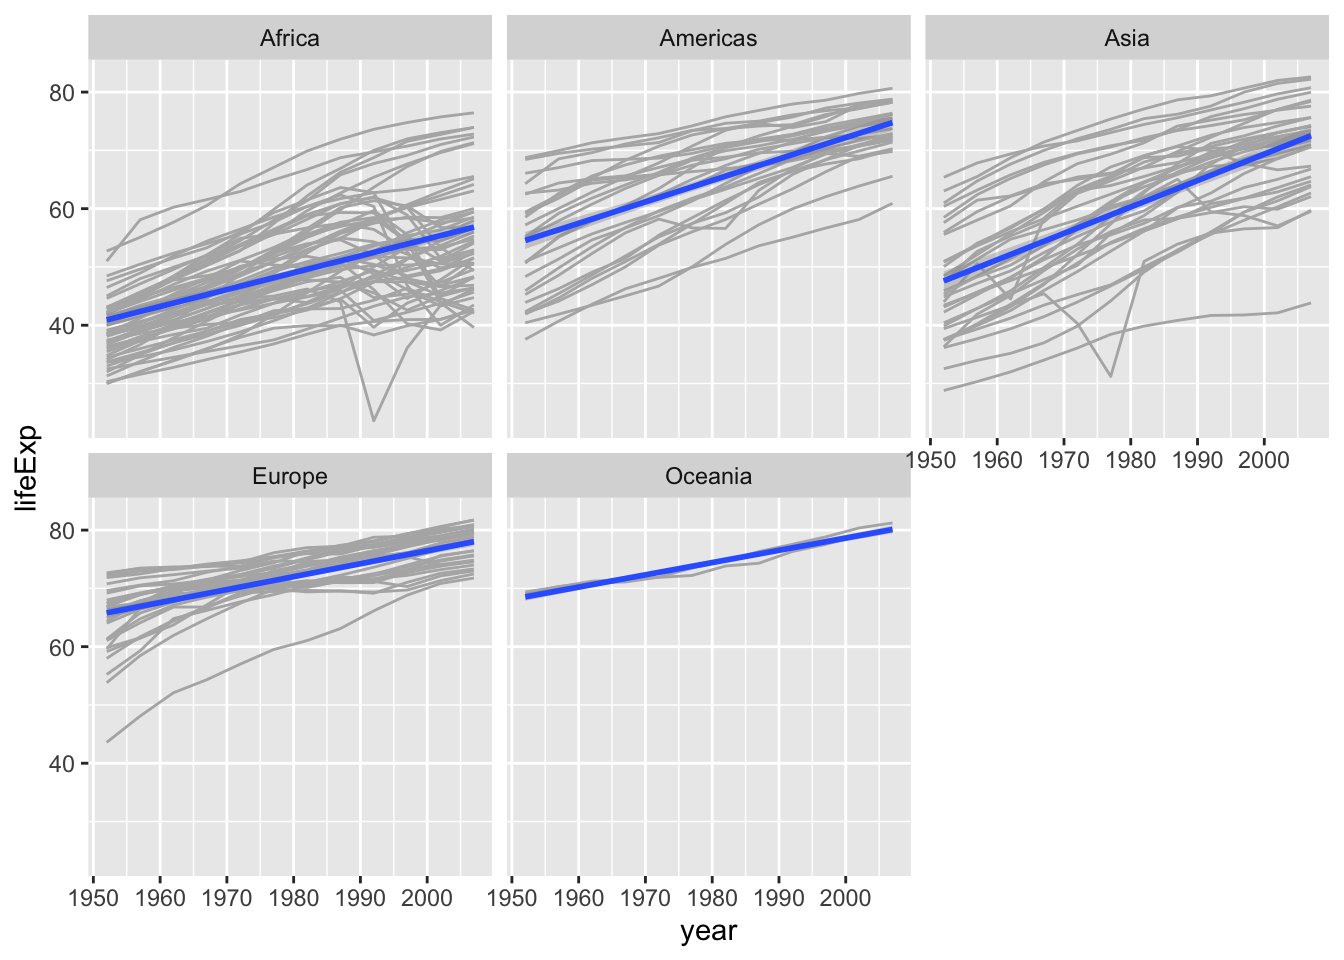
\includegraphics[scale=0.5]{practica3-img-gapminder-lifeExp.png}
\end{center}
\end{enumerate}

\item (De ac\'a en adelante, trabajar con el dataset \lstinline{penguins} disponible en la biblioteca \lstinline{seaborn}).
?`Cu\'antas
filas y
columnas hay en el dataset penguins?

\begin{lstlisting}
import seaborn as sns
penguins = sns.load_dataset("penguins")
\end{lstlisting}

\begin{center}
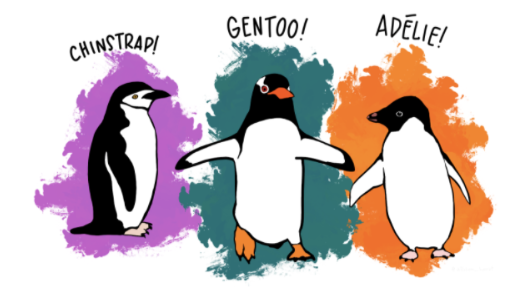
\includegraphics[scale=0.5, align=c]{practica3-img-penguins_species.png}
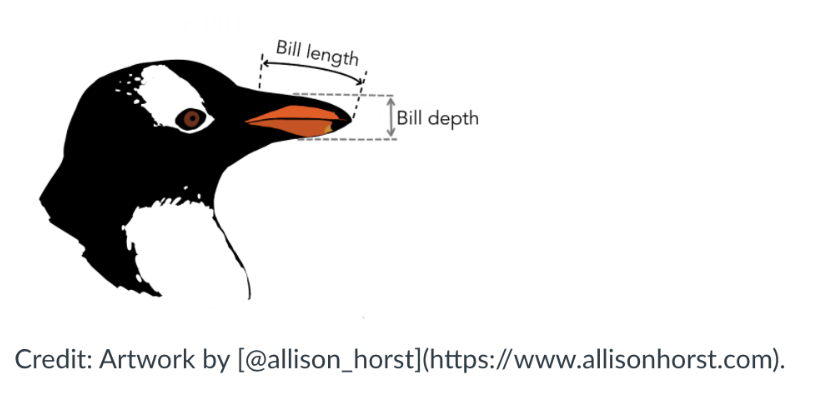
\includegraphics[scale=0.3, align=c]{practica3-img-penguins_bill.png}
\end{center}

\item
Como vimos en el Ejercicio \ref{ej:map}, si asignamos una codificación (o mapeo) al definir un \lstinline{Plot()}, el mapeo se asigna en todas las capas de marcas (objetos mark). En cambio, si asignamos una codificación dentro del método \lstinline{add()} de una marca, mapeo se realiza solo en esa capa. Por último, si asignamos un parámetro de la marca, el valor se asigna directamente (ver gráfico).

\begin{center}
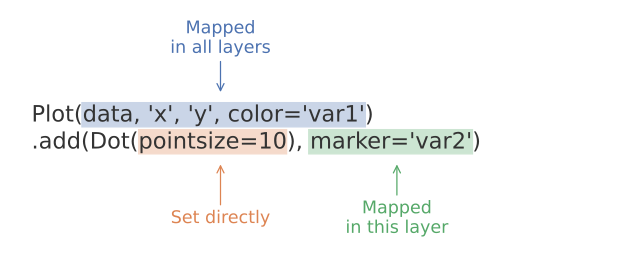
\includegraphics[scale=0.5, align=c]{practica3-img-mappings.png}
\end{center}


?`Qu\'e resultado esperan para el siguiente gráfico? ?`Cu\'ales codificaciones se pasan de \lstinline{Plot()} a \lstinline{Dot()} y cuáles no pueden pasarse? ¿Cuáles codificaciones se establecen en \lstinline{Dot()}? ¿Cuáles variables están asignadas directamente en \lstinline{Dot()}? ¿De qué color van a pintarse los puntos?



\begin{lstlisting}
(
    so.Plot(
        penguins, x="bill_length_mm", y="bill_depth_mm",
        edgewidth="body_mass_g", marker = "species",
        linestyle = "island", color = "species"
    )
    .add(so.Dot(color=".8"), edgecolor="sex")
)
\end{lstlisting}

\item 
\begin{enumerate}
\item ¿Cuántos pingüinos hay en cada isla en la base de datos? Recordar los comandos \lstinline{groupby()} y \lstinline{size()} de la práctica anterior.
\item Realizar un grafico de barras con la cantidad de pingünos en cada isla, completando el siguiente código.
\begin{lstlisting}
pinguinos_por_isla = penguins.???   # Usar el codigo del item anterior.
(
    so.Plot(x=pinguinos_por_isla.index, y=???)
    .add(so.Bar())
)
\end{lstlisting}
\item El gráfico que acabamos de hacer es un histograma categórico (usamos una variable categórica en el eje X). Podemos realizar el mismo gráfico usando la función \lstinline{Hist()} para contar automáticamente las cantidades (sin definir una variable \lstinline{pinguinos_por_isla}. Completar el siguiente código.
\begin{lstlisting}
(
    so.Plot(data = penguins, x=island)
    .add(so.Bar(), so.Hist())
)
\end{lstlisting}
\item ¿Por qué no especificamos ninguna variable $y$ en el último gráfico?
\item Queremos ver en un gráfico cuántos pingüinos de cada especie hay en cada isla, ¿cómo podemos hacerlo? Si usan un gráfico de barras, pueden utilizar la función \lstinline{dodge()} para hacer varias barras por categoría.
\item ¿Cómo podrían visualizar lo mismo usando \lstinline{facet()}?
\end{enumerate}

\item Realizar un histograma de la cantidad de pingüinos en función del tamaño del ala (variable \lstinline{flipper_length_mm}). A partir del gráfico, estimar el valor mínimo, máximo, la media y la mediana. Verificar sus estimaciones utilizando los comandos apropiados.

\item \label{depthvslength}
\begin{enumerate}
\item Hacer un \lstinline{scatterplot} de \lstinline{bill_depth_mm} (en el eje $y$) vs. \lstinline{bill_length_mm} (en el eje $x$).
\item ¿Distinguen grupos distintos de puntos en el gráfico? ¿A qué puede deberse?
\item Introducir alguna modificación en el gráfico anterior para verificar o refutar su conjetura del ítem anterior.
\end{enumerate}

\item \begin{enumerate}
\item Calcular distintos estadísticos de la variable \lstinline{bill_depth_mm} (mínimo, máximo, media, ...).
\item Según lo observado en el ejercicio anterior, ¿esos valores varían según la especie? ¿Cómo podemos usar gráficos BoxPlot para para ver la relaci\'on entre \lstinline{species} y \lstinline{bill_depth_mm}?
\end{enumerate}

\item
\begin{enumerate}
\item Rehacer el scatter plot del ejercicio \ref{depthvslength}, coloreando los puntos según el sexo. ¿Qué se observa?
\item Usando la función \lstinline{facet()} separar el gráfico del item anterior en tres subgráficos, uno para cada especie.
\end{enumerate}

%\item Agregar un ``caption'' al gr\'afico de arriba. Ayuda: Mirar la documentaci\'on de \lstinline{labs()}.
\item 
\begin{enumerate}
\item Rehacer el scatter plot del ejercicio \ref{depthvslength}, modificando el tamaño de los puntos según el peso de cada pingüino, utilizando el parámetro \lstinline{pointsize="???"}. ¿Qué se observa?
\item En base a lo observado, ¿cuál es la especie con mayor peso? Verificarlo mediante alguna visualización.
\end{enumerate}


\end{enumerate}

\end{document}


\item Recrear la siguiente visualizaci\'on. ?`A qu\'e aes deber\'ia mapearse \lstinline{bill_depth_mm}? ?`El mapeo debe ser global o local?
\begin{center}
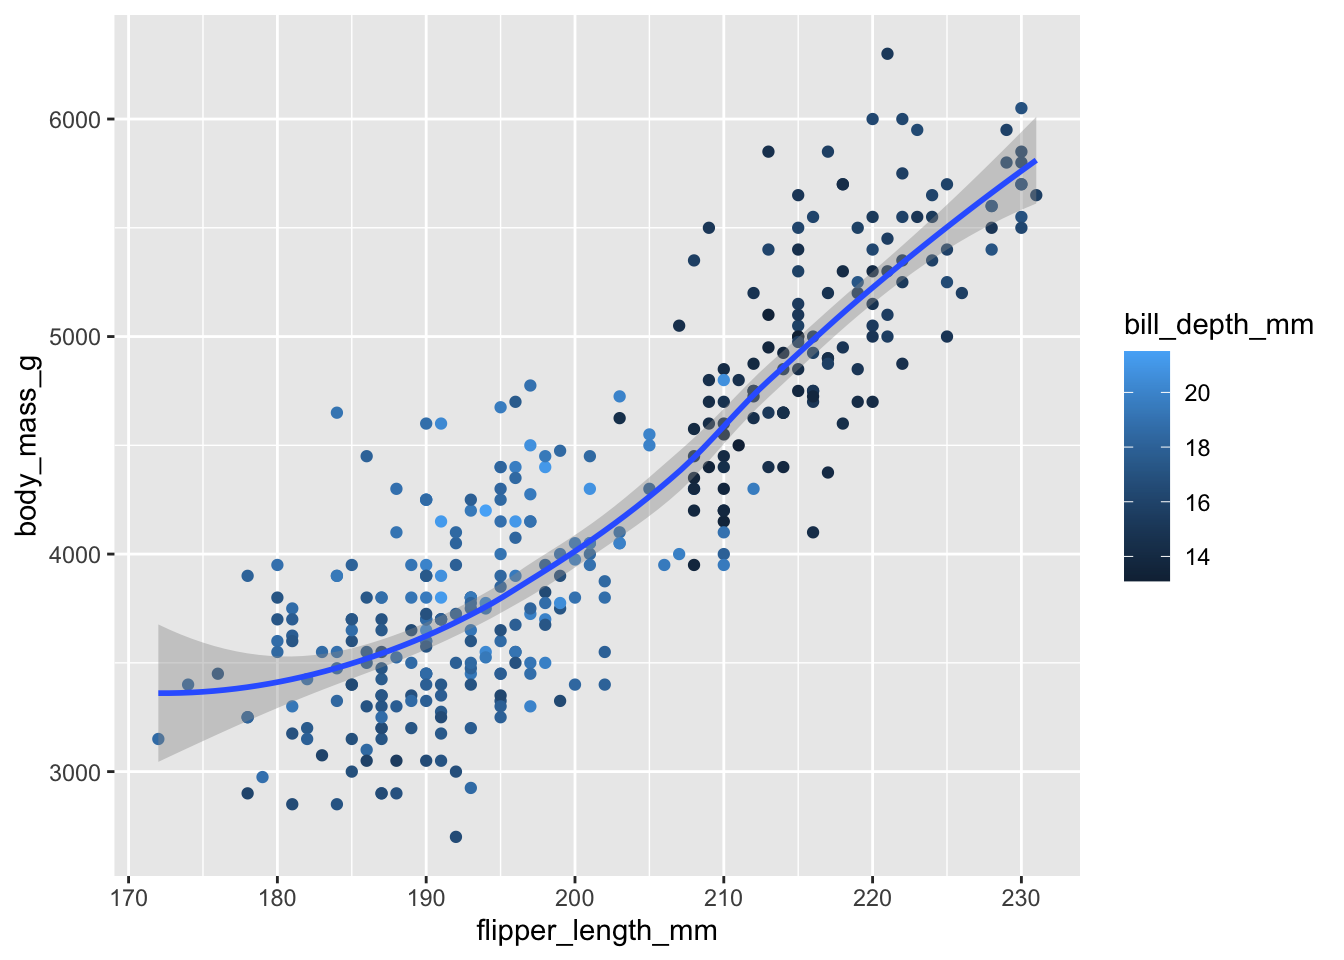
\includegraphics[scale=0.3]{practica3-img-penguins-mass.png}
\end{center}

\item Sin correr el c\'odigo, predecir qu\'e gr\'afico produce.
\begin{lstlisting}
ggplot(data = penguins,
       mapping = aes(x = flipper_length_mm, y = body_mass_g, color = island) ) +
  geom_point() +
  geom_smooth(se = FALSE)
\end{lstlisting}

\item Sin correr el c\'odigo, ?`estos dos gr\'aficos van a ser iguales o diferentes? ?`Por qu\'e?
\begin{lstlisting}
# grafico 1
ggplot(
  data = penguins,
  mapping = aes(x = flipper_length_mm, y = body_mass_g)
) +
  geom_point() +
  geom_smooth()

# grafico 2
ggplot() +
  geom_point(
    data = penguins,
    mapping = aes(x = flipper_length_mm, y = body_mass_g)
  ) +
  geom_smooth(
    data = penguins,
    mapping = aes(x = flipper_length_mm, y = body_mass_g)
  )
\end{lstlisting}

\item Sin correr el c\'odigo, predecir qu\'e gr\'afico produce.
\begin{lstlisting}
ggplot(data = penguins,
       mapping = aes(x = flipper_length_mm, y = body_mass_g, color = island) ) +
  geom_point() +
  geom_smooth(se = FALSE)
\end{lstlisting}

\item Sin correr el c\'odigo, ?`estos dos gr\'aficos van a ser iguales o diferentes? ?`Por qu\'e?
\begin{lstlisting}
# grafico 1
ggplot(
  data = penguins,
  mapping = aes(x = flipper_length_mm, y = body_mass_g)
) +
  geom_point() +
  geom_smooth()

# grafico 2
ggplot() +
  geom_point(
    data = penguins,
    mapping = aes(x = flipper_length_mm, y = body_mass_g)
  ) +
  geom_smooth(
    data = penguins,
    mapping = aes(x = flipper_length_mm, y = body_mass_g)
  )
\end{lstlisting}


FACTORES


%%\item Las variables de clase "factor" (factores, o fct) son una clase especial que tiene R para trabajar con variables categ\'oricas. Una vez que se crean, los factores s\'olo pueden contener un conjunto pre-definido de valores que se conocen como los niveles del factor. ?`Qu\'e variables del dataset de gapminder son factores?
%
%\item Redefinir niveles. Supongamos que queremos cambiar la denominaci\'on del continente de Argentina a ``America'' (sin la s final). Prueben lo siguiente. ?`Qu\'e pas\'o? ?`Por qu\'e no funciona?
%\begin{lstlisting}
%class(gm.sur$continent)
%gm.sur$continent <- "America"
%class(gm.sur$continent)
%\end{lstlisting}
%
%Ahora prueben esto. ?`Entienden por qu\'e funciona?
%
%levels(gm.sur$continent) <- c("Africa", "America", "Asia", "Europe", "Oceania")
%class(gm.sur$continent)
%head(gm.sur)
%
%\item  Vamos a usar mucho "factores" a lo largo del curso, pero para que se den una idea, por ejemplo, los factores son muy \'utiles para codificar variables categ\'oricas en gr\'aficos. Vamos a ver esto bastante a lo largo de las clases, pero para que vean una aplicaci\'on simple, corran estas l\'ineas usando el paquete (que vamos a ver en las pr\'oximas clases) ggplot2.
%
%library(ggplot2)
%
%ggplot(data = gm.sur,
%       mapping = aes(x = year, y = pop, col = country)) +
%  geom_point(size = 3) +
%  theme_classic()
%
%Ahora corran lo siguiente. ?`En qu\'e difiere del anterior? ?`Pueden intuir por qu\'e tenemos ese resultado?
%
%ggplot(data = gm.sur,
%       mapping = aes(x = year, y = pop, size = country)) +
%  geom_point() +
%  theme_classic()
%
%?`Y si reemplazan size por shape dentro de aes(...)?
%
%4.13. Cambien m\'as cosas del c\'odigo anterior y prueben el resultado. De hecho, cambiar cosas y ver qu\'e pasa es una gran forma de aprender.

